\documentclass[12pt]{article}
\usepackage[T2A]{fontenc}
\usepackage[utf8]{inputenc} 
\usepackage[english,russian]{babel} 
  
\usepackage{amsmath} 
\usepackage{listings}
\usepackage{graphicx}
\DeclareGraphicsExtensions{.pdf,.png,.jpg}
\usepackage{amssymb}
\usepackage{float}
\usepackage{amsthm}

\newtheorem{claim}{Утверждение}
\newtheorem*{claim*}{Утверждение}

{\tiny }\begin{document}
	\begin{center}
		\Large \textbf{Алгоритм принятия решения о существовании пути в лабиринте.\\}
		\normalsize 
		\bigskip
		Составитель задачи: Яроцкий Дмитрий Александрович, и.о. заведующего сектором 10.1 ИППИ им. А.А. Харкевича РАН\\
		Задачу решил студент второго курса ФУПМ -- Чеканов Михаил.\\
	\end{center}
\section*{Формулировка задачи}
	Рассмотрим квадратный лабиринт размера $n \times n$, понимая под ним сетку из ячеек, у каждой из которых некоторые из 4 стенок открыты, а остальные закрыты. Нас будет интересовать такая задача: для заданных двух ячеек A и B определить, существует ли проход от A до B. Будем считать, что проход предъявлять не нужно, предполагается лишь ответ в форме «да/нет».

Такую задачу можно решить простым последовательным алгоритмом обхода всех ячеек, соединенных с данной, однако он может потребовать $O(n^2)$ шагов (если путь заполняет почти весь лабиринт). Вопрос: можно ли решить эту задачу быстрее, например за $O(n)$ или даже $o(n)$ шагов, с помощью клеточного автомата (т. е. параллельных вычислителей, локализованных в ячейках сетки и общающихся с ближайшими соседями)?

Решение с помощью клеточного автомата (КА) подразумевает три составные части:

\begin{itemize}
\item инициализация КА: предварительное отображение ячеек лабиринта в начальные состояния вычислителей на основании информации о связях ячейки с ближайшими соседями и принадлежности к ячейкам $A, B$;
\item собственно правила итерации КА, т.е. закон изменения состояний вычислителей в зависимости от собственных состояний и состояний ближайших соседей (одновременное однократное изменение состояний всех вычислителей считается за один шаг алгоритма);
\item условия принятия окончательного решения о наличии/отсутствии прохода между $A$ и $B$ — можно считать, что решение принимается, когда либо все вычислители (конъюнктивный вариант), либо хотя бы один (дизъюнктивный вариант) переходят в некоторые выделенные состояния.
\end{itemize}

\bigskip
 
 В данной работе будет предъявлен алгоритм, решающий данную задачу за $O(n)$ итераций КА и доказана принципиальная невозможность существования алгоритма, работающего за $o(n)$
 
Вначале приведём упомянутый алгоритм.
 
\section*{Описание клеточного автомата}
\subsection*{Состояния ячейки}
В каждой ячейке будем хранить информацию о возможности перейти в соседние клетки, а также является ли стартом(в дальнейшем клетка $A$), финишем(клетка $B$) или ни тем, ни другим.\\

Для кодирования данной информации потребуется $6$. Условимся кодировать состояние автомата следующим образом:

\begin{itemize}
\item $0$-й бит равен $1$, если данная клетка -- клетка $A$;
\item $1$-й бит равен $1$, если данная клетка -- клетка $B$;
\item $2$-й бит равен $1$, если данная клетка имеет стенку сверху;
\item $3$-й бит равен $1$, если данная клетка имеет стенку справа;
\item $4$-й бит равен $1$, если данная клетка имеет стенку снизу;
\item $5$-й бит равен $1$, если данная клетка имеет стенку слева;
\end{itemize}

Схематичное изображение битов и кодируемых им объектов изображено на рис.\ref{fig:bits}. На рис.\ref{fig:bits_ex} приведён пример кодировки состояний автомата.


  \begin{minipage}{\linewidth}
      \centering
      \begin{minipage}{0.4\linewidth}
          \begin{figure}[H]
              \includegraphics[width=\linewidth]{draw1}
              \caption{Связь элементов ячейки с битами}
              \label{fig:bits}
          \end{figure}
      \end{minipage}
      \hspace{0.15\linewidth}
      \begin{minipage}{0.4\linewidth}
          \begin{figure}[H]
              \includegraphics[width=\linewidth]{draw2}
              \caption{Пример кодировки ячеек лабиринта}
              \label{fig:bits_ex}
          \end{figure}
      \end{minipage}
  \end{minipage}

Отметим что, кодировка начальных состояний однозначно определяет стенки в лабиринте, поэтому изменение состояний автоматов можно рассматривать как изменение конфигурации лабиринта.

В качестве инициализации клеточного автомата понимаем задание состояния автоматов в ячейках в соответствии с заданной схемой лабиринта.

Отметим, что мы несколько модифируем данный нам алгоритм. А именно, заключим его в "кожух" из пустых клеток. Это необходимо, для того, чтобы правила, которые мы приведём ниже работали и для граничных клеток лабиринта(такая конструкция гарантирует наличие всех соседей у каждой клетки исходного лабиринта)

\subsection*{Правила изменений состояний автоматов}

Как отмечалось в конце предыдущего пункта изменения состояний автоматов можно рассматривать как преобразование лабиринта, поэтому далее будем говорить о добавлении/удалении стенок и перемещение точек старта/финиша, подразумевая соответствующие изменения состояний автоматов.\\
Cписок правил следующий:
\begin{itemize}
	\item[$1$] Если клетка содержит одиночную стенку (то есть такая стенка, что хотя бы с одного конца, она не соединена ни с одной стенкой)и при этом клетки содержащие , удалить эту стенку.
	\item[$2$] Если клетка содержит левый-верхний уголок, добавить в эту клетку нижний правый уголок. Если помимо этого из левой клетки можно перейти в левую верхнюю, то удаляем левую стенку, аналогично, если  из верхней можно перейти в  левую верхнюю удаляем верхнюю стенку.
	\item[$3$] Если клетка содержит старт/финиш, и из неё есть путь вниз, сместить вниз -- в противном случае, если возможно, сместить вправо(если нельзя и этого, оставить без изменений)
\end{itemize}

Для нагляlности на(рис. \ref{fig:r1}, \ref{fig:r2}, \ref{fig:r3}) продемонстрированы применения этих правил.

		  \begin{figure}[H]
		  	  \centering
              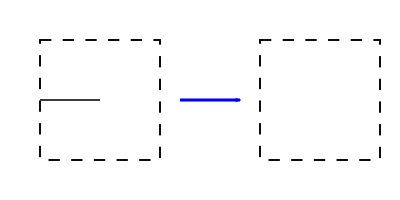
\includegraphics[width=0.4\linewidth]{rule1}
              \caption{Правило 1}
              \label{fig:r1}
          \end{figure}
          \begin{figure}[H]
          \centering
              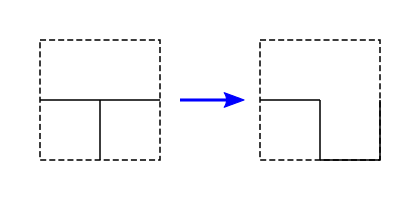
\includegraphics[width=0.4\linewidth]{rule2}
              \caption{Правило 2}
              \label{fig:r2}
          \end{figure}
          \begin{figure}[H]
          \centering 
              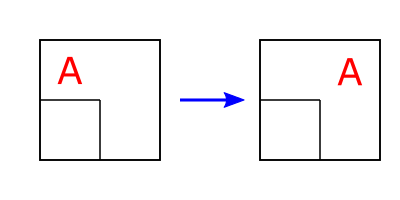
\includegraphics[width=0.4\linewidth]{rule3}
              \caption{Правило 3}
              \label{fig:r3}
          \end{figure}
          
\subsection*{Условия окончания работы и принятия решения}

Автомат прекращает работу, если в одной из ячеек $0$-й и $1$-й биты равны $1$. В этом случае старт совпадёт с финишем, что означает существование пути в исходном лабиринте.\\

Автомат также прекратит работу, если старт/финиш окажется в изолированной клетке. В этом случае пути нет.\\

Далее будет показано, что такой клеточный автомат позволяет "свернуть" лабиринт, так, что если старт и финиш располагались в одной компоненте связности, то в преобразованном лабиринте они окажутся в одной клетке. В противном случае старт или финиш окажется в изолированной клетке.

\section*{Пример работы алгоритма}

Для наглядности приведём примеры работы клеточного автомат в виде схем лабиринтов, соответствующих состояниям клеток на каждом такте. 

Первый пример(рис. \ref{fig:ex_1})) иллюстирирует решение на лабиринте, на котором алгоритм обхода в глубину работает за $O(n^2)$.

\begin{figure}[H]
	\begin{minipage}[h]{0.32\linewidth}
		\center{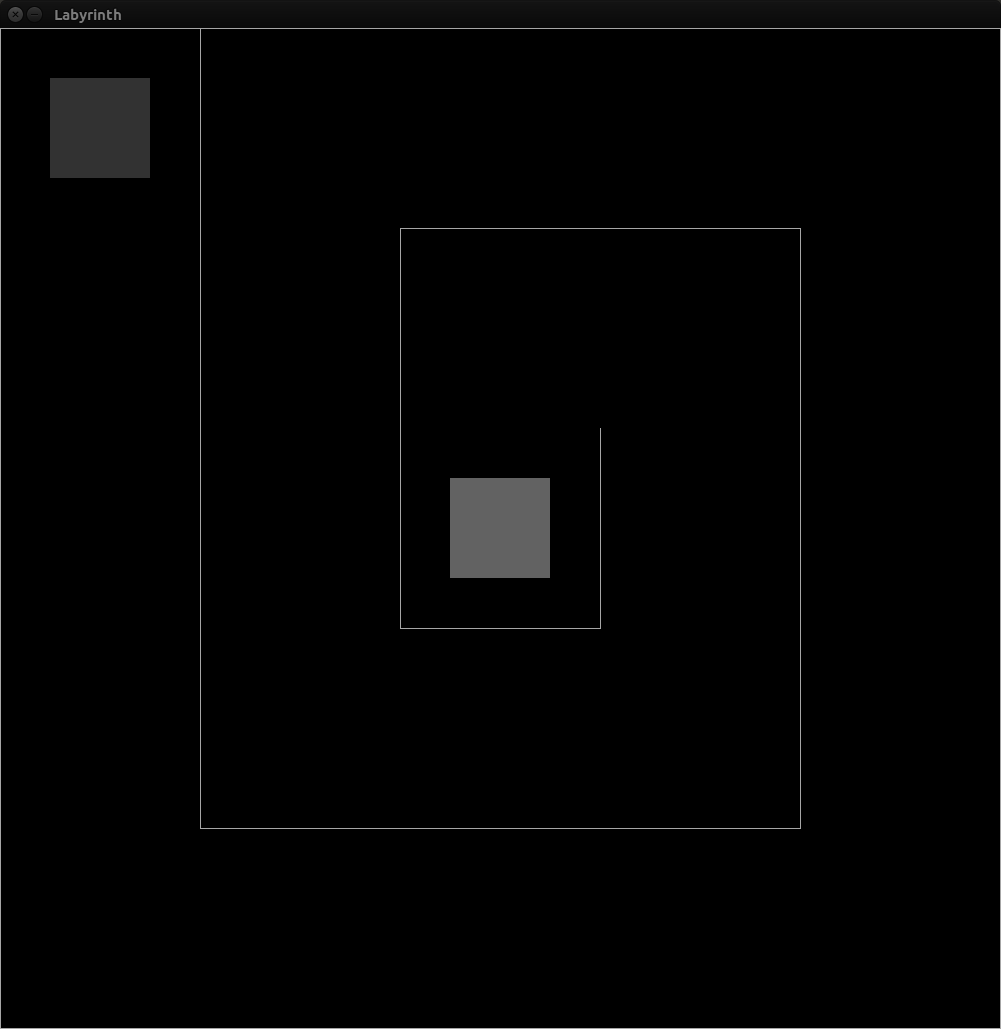
\includegraphics[width=1\linewidth]{1-1}}\\
	\end{minipage}
	\hfill
	\begin{minipage}[h]{0.32\linewidth}
		\center{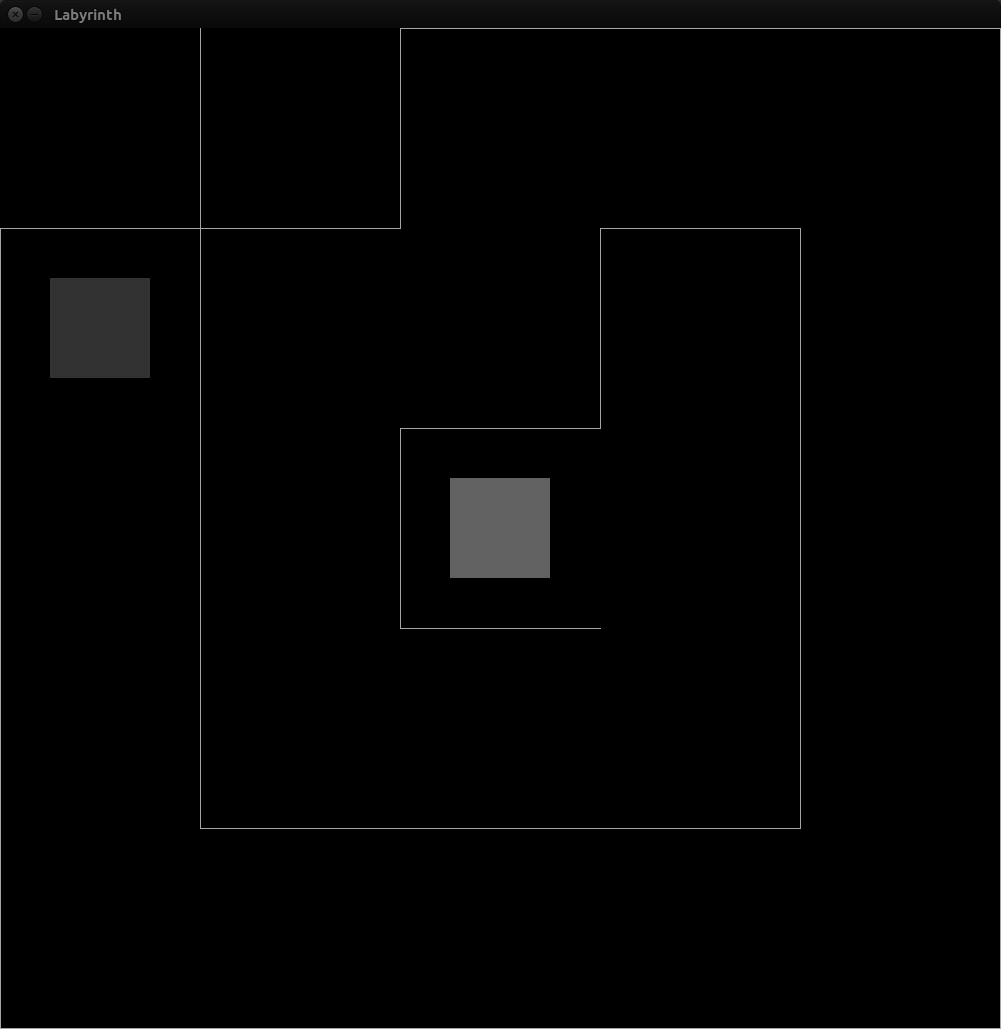
\includegraphics[width=1\linewidth]{1-2}}\\
	\end{minipage}
	\hfill
	\begin{minipage}[h]{0.32\linewidth}
		\center{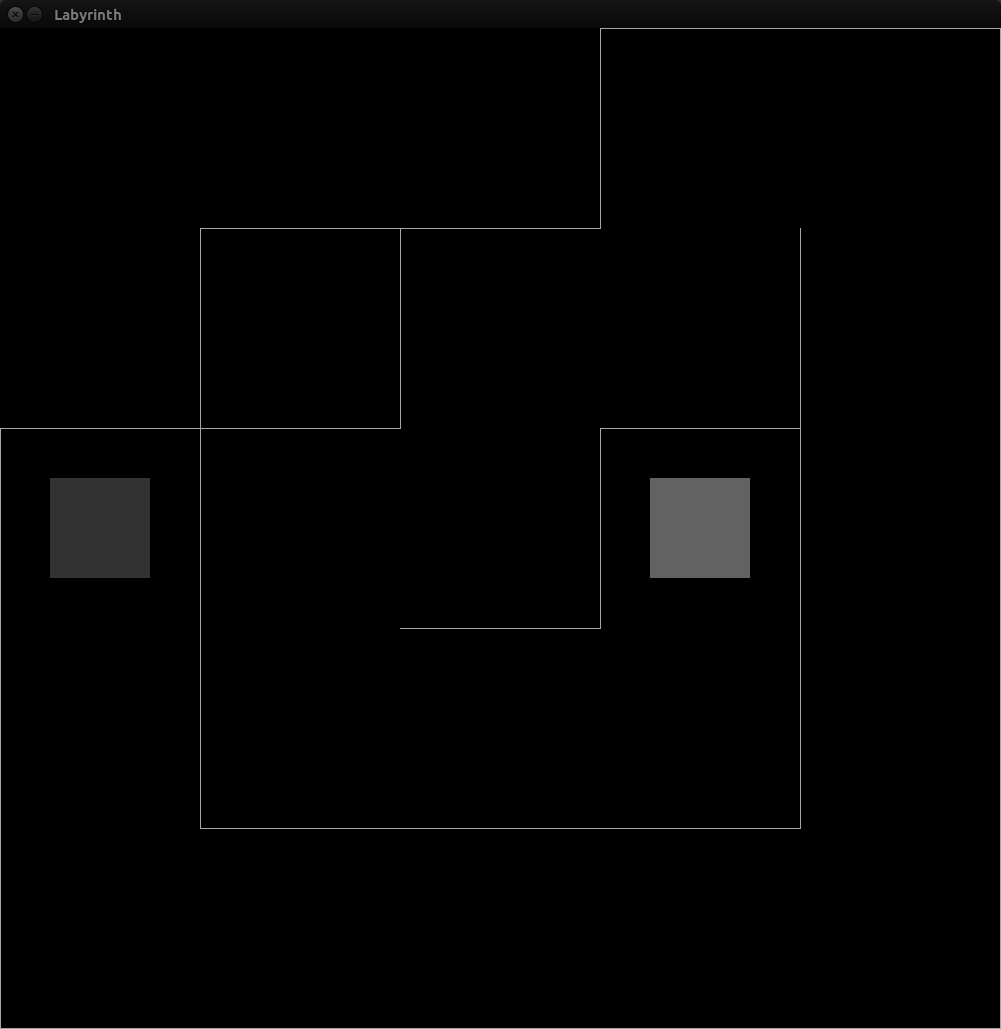
\includegraphics[width=1\linewidth]{1-3}}\\
	\end{minipage}
	\hfill
	\begin{minipage}[h]{0.32\linewidth}
		\center{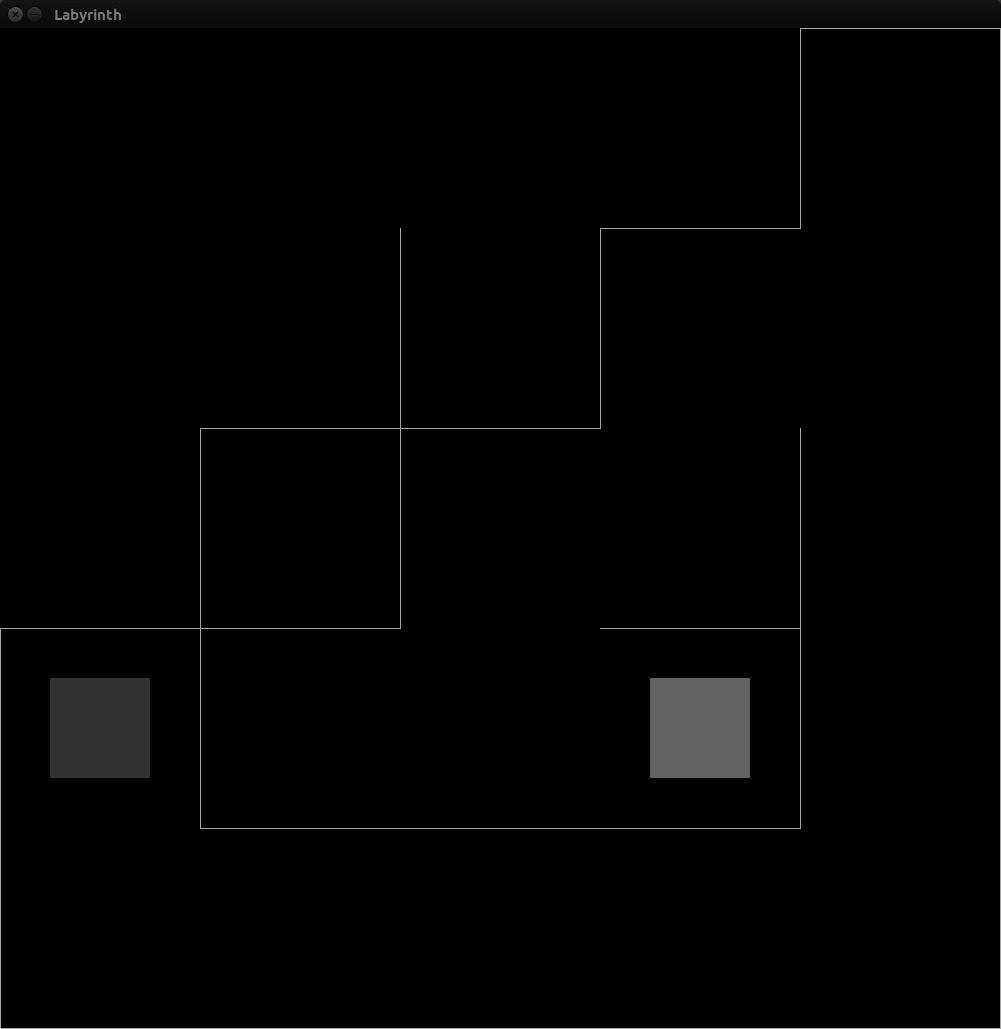
\includegraphics[width=1\linewidth]{1-4}}\\
	\end{minipage}
	\hfill
	\begin{minipage}[h]{0.32\linewidth}
		\center{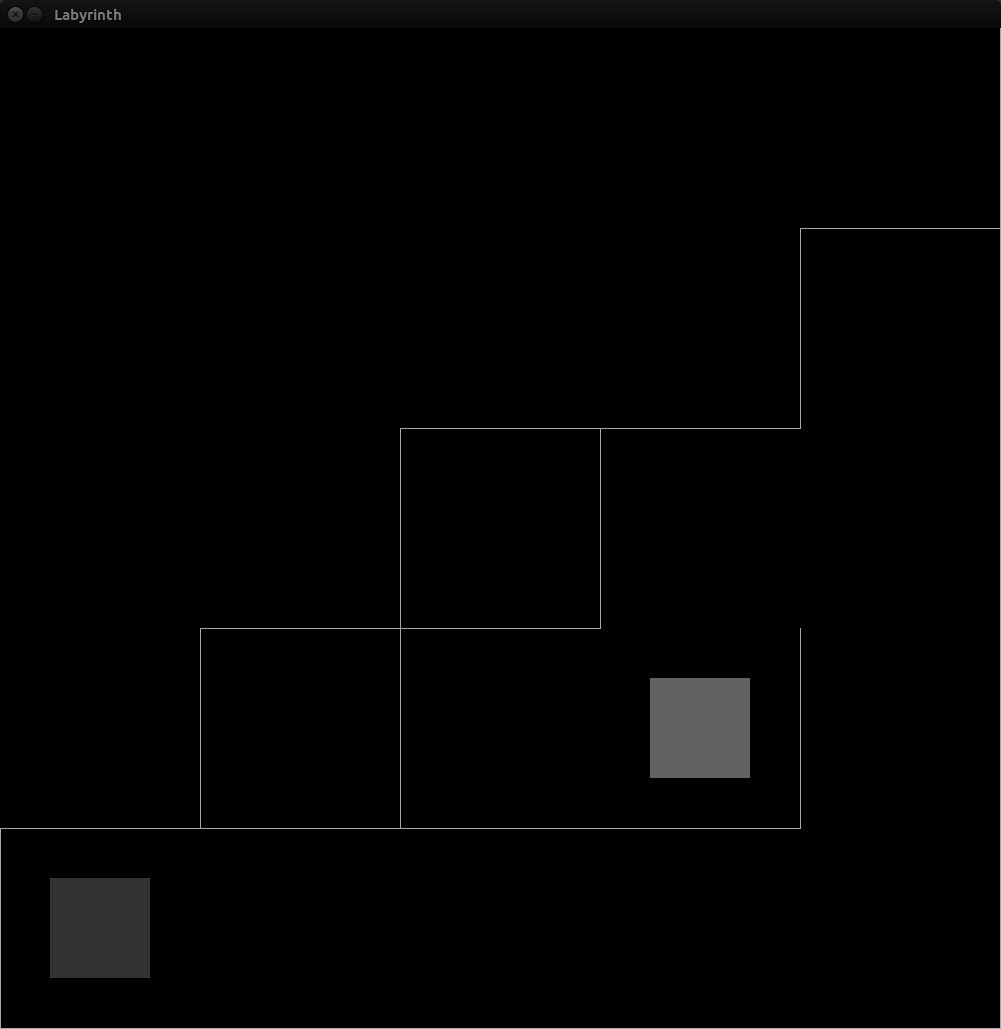
\includegraphics[width=1\linewidth]{1-5}}\\
	\end{minipage}
	\hfill
	\begin{minipage}[h]{0.32\linewidth}
		\center{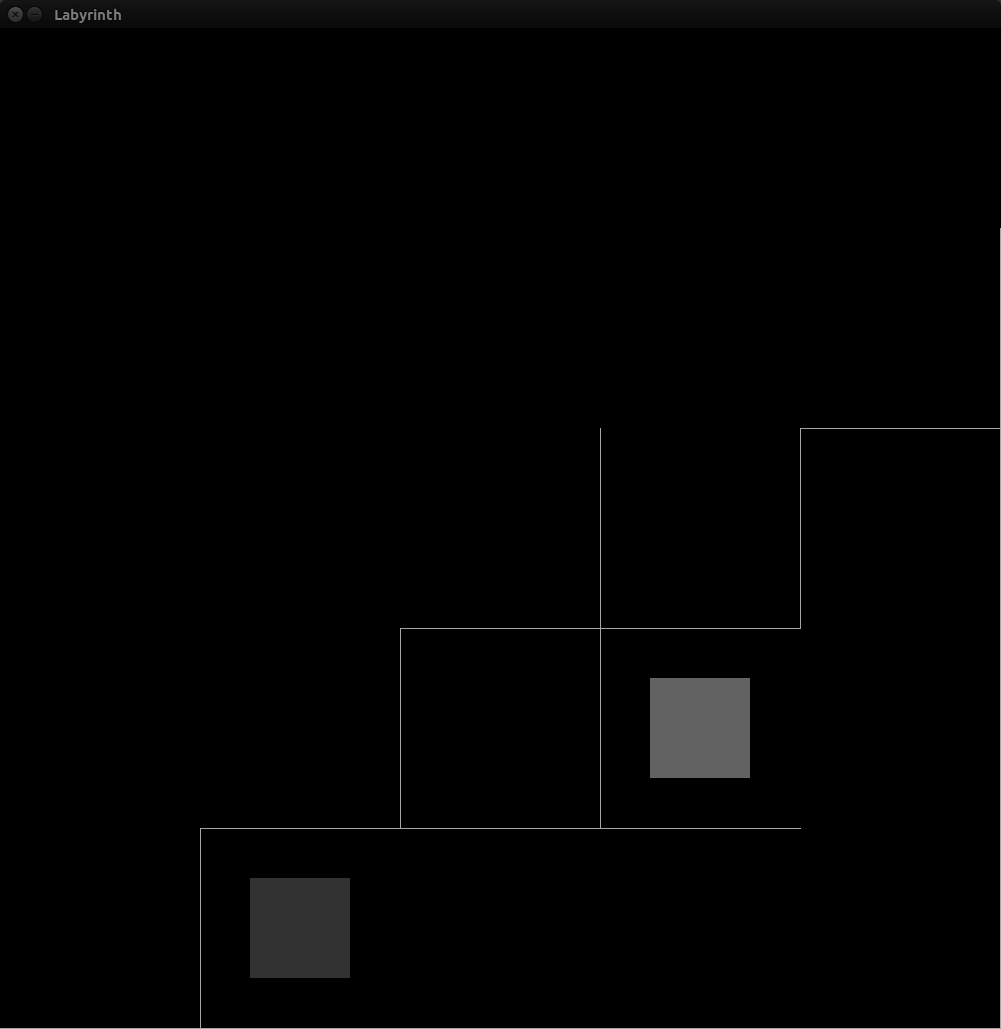
\includegraphics[width=1\linewidth]{1-6}}\\
	\end{minipage}
	\hfill
	\begin{minipage}[h]{0.32\linewidth}
		\center{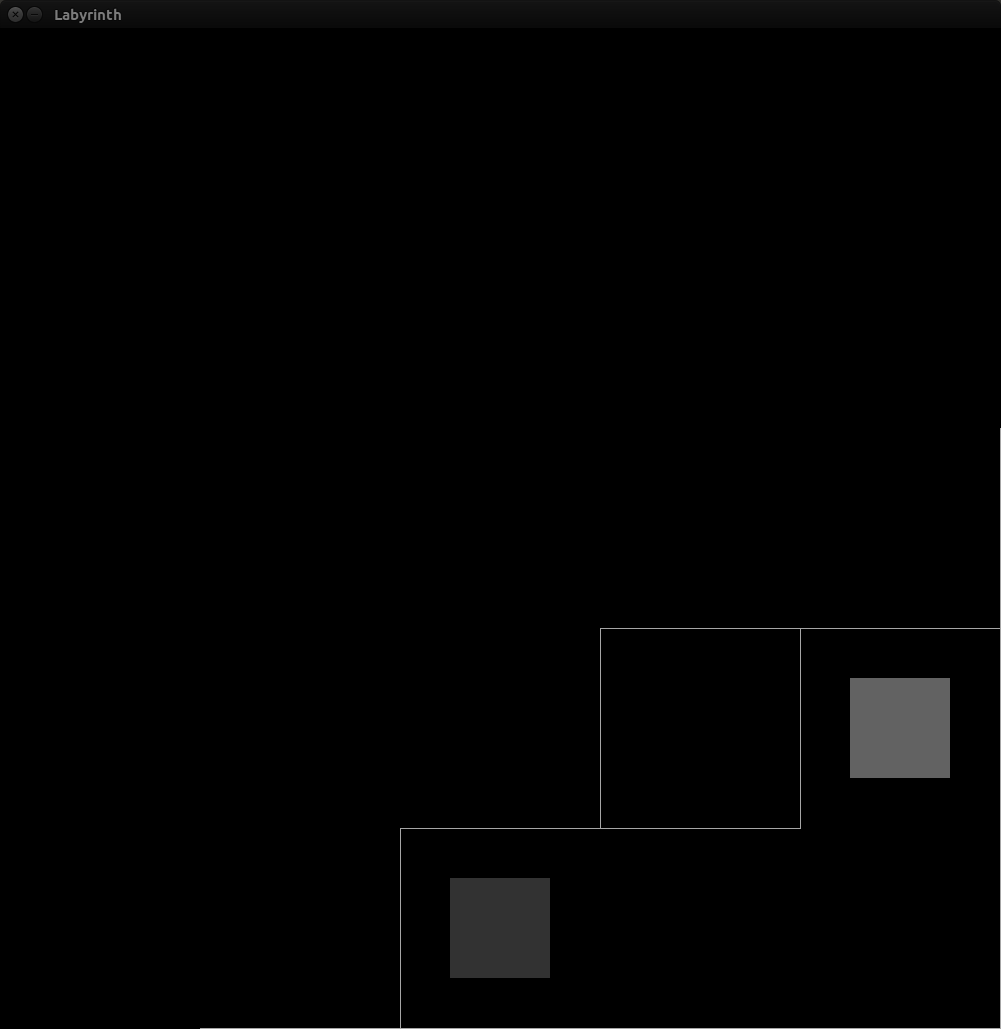
\includegraphics[width=1\linewidth]{1-7}}\\
	\end{minipage}
	\hfill
	\begin{minipage}[h]{0.32\linewidth}
		\center{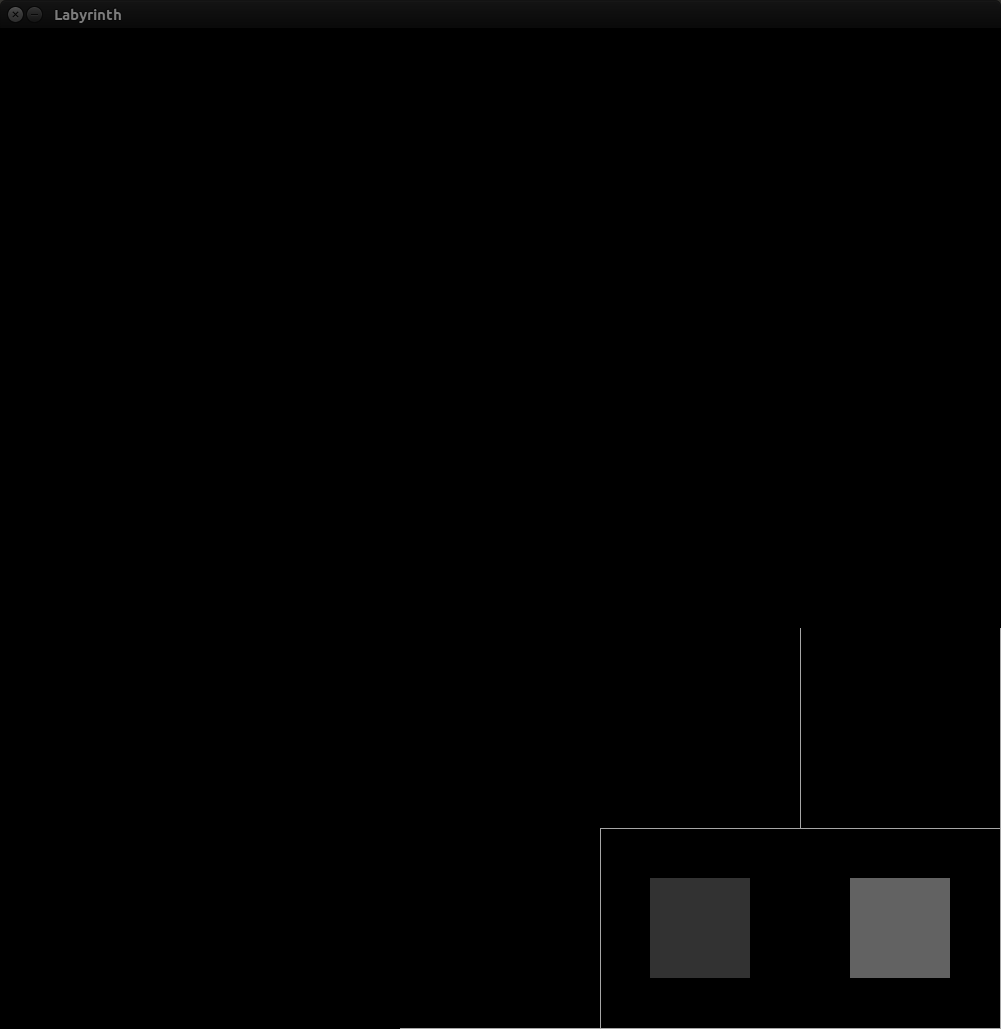
\includegraphics[width=1\linewidth]{1-8}}\\
	\end{minipage}
	\hfill
	\begin{minipage}[h]{0.32\linewidth}
		\center{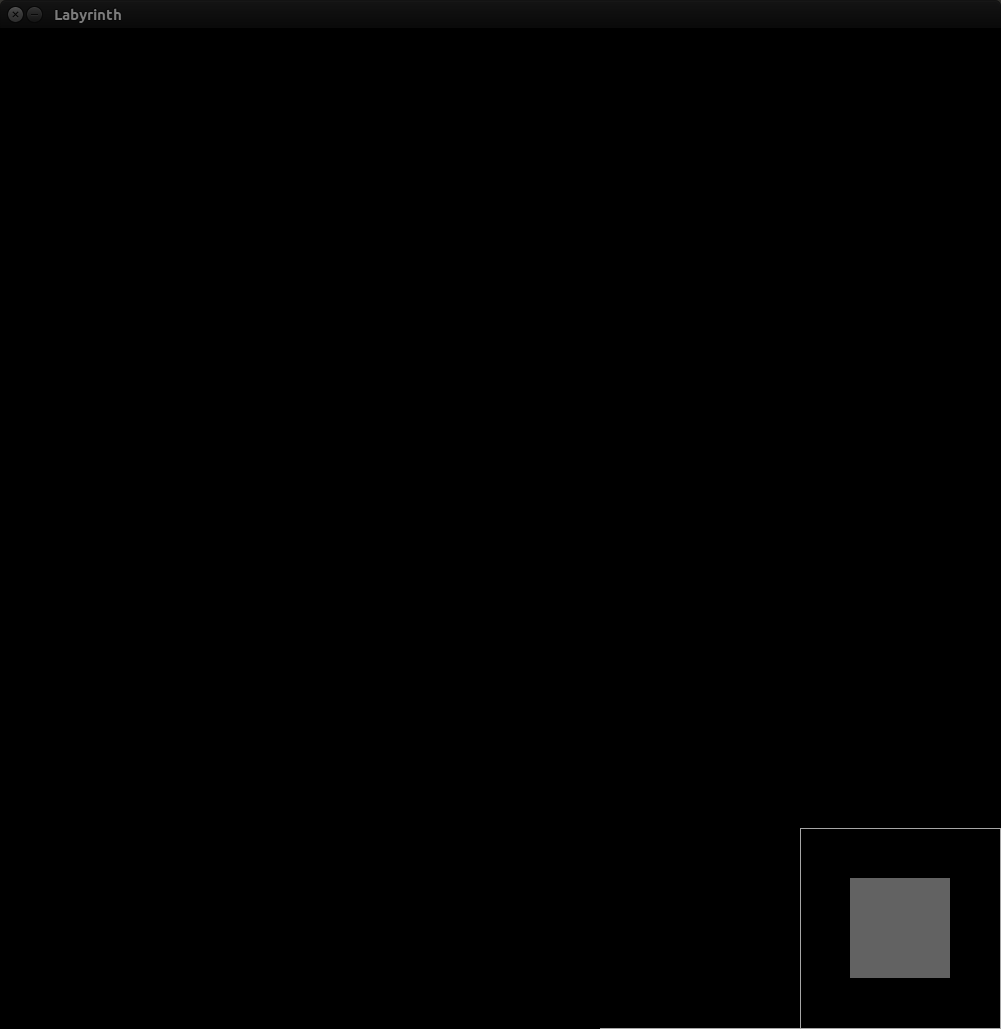
\includegraphics[width=1\linewidth]{1-9}}\\
	\end{minipage}
	\hfill
	\caption{Пример работы алгоритма(Путь есть)}
	\label{fig:ex_1}
\end{figure}

Второй пример(рис. \ref{fig:ex_2}) иллюстрирует работу на лабиринте, где не существует пути из $A$ в $B$

\begin{figure}[H]
	\begin{minipage}[h]{0.3\linewidth}
		\center{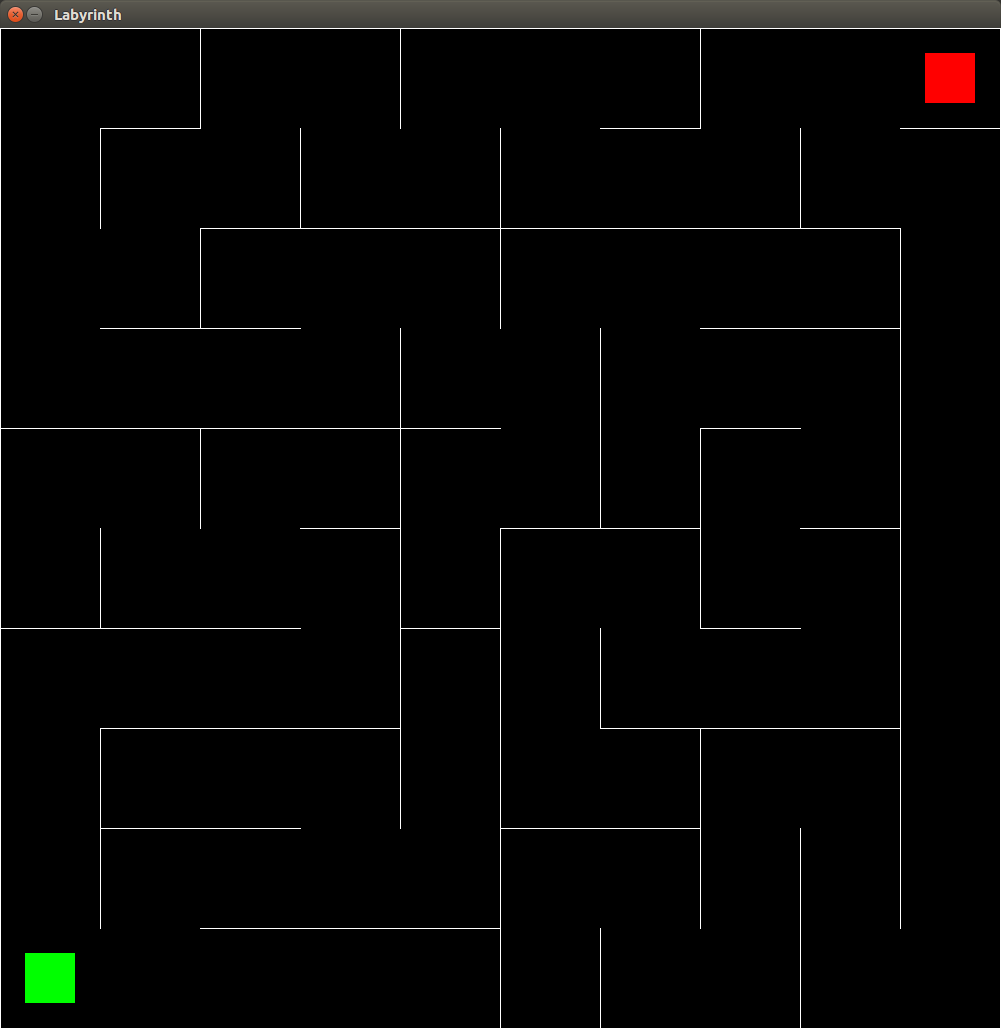
\includegraphics[width=1\linewidth]{2-1}}\\
	\end{minipage}
	\hfill
	\begin{minipage}[h]{0.3\linewidth}
		\center{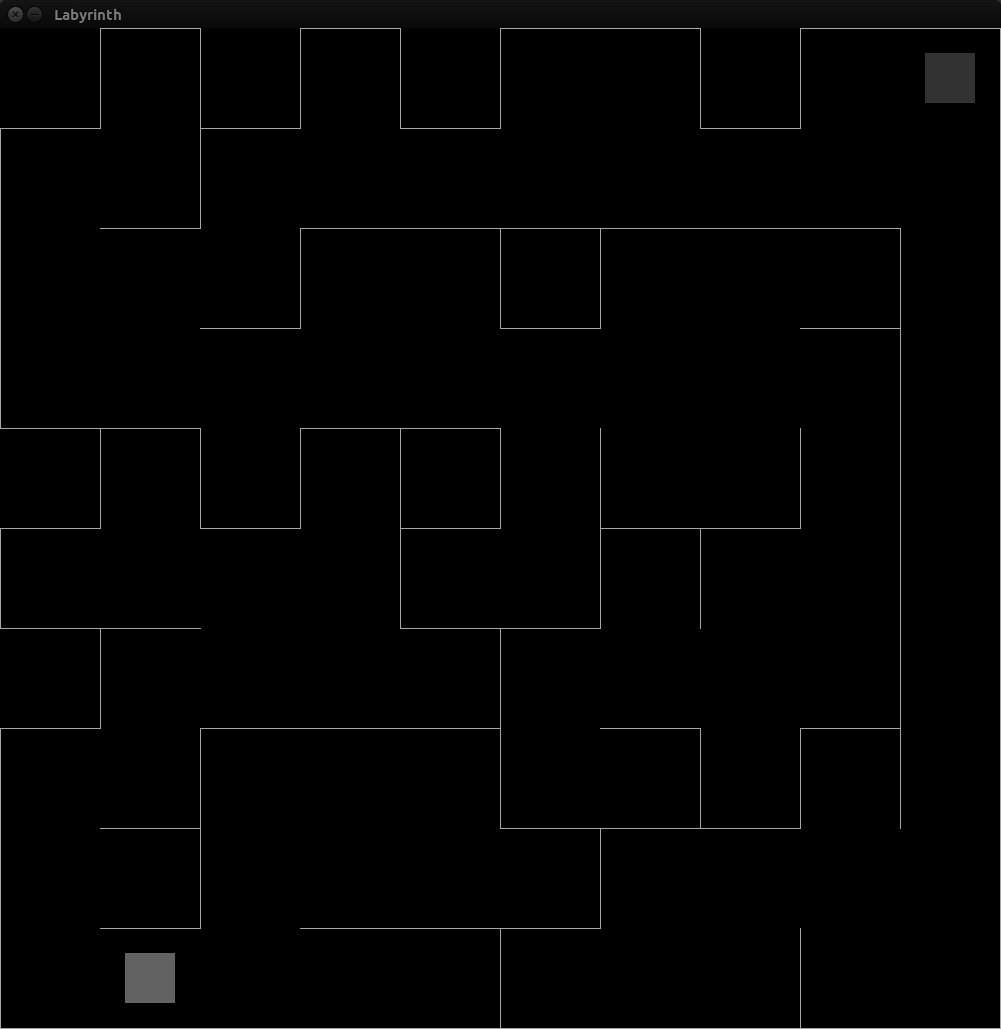
\includegraphics[width=1\linewidth]{2-2}}\\
	\end{minipage}
	\hfill
	\begin{minipage}[h]{0.3\linewidth}
		\center{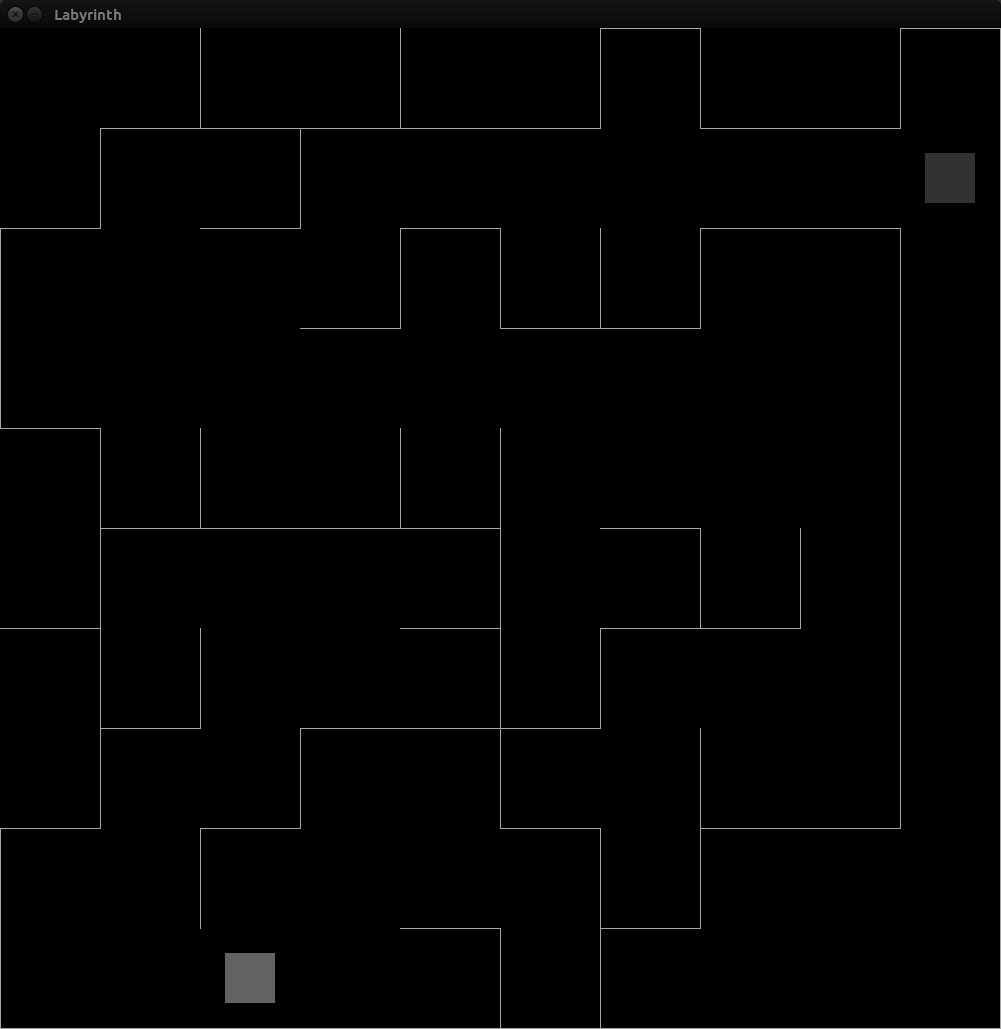
\includegraphics[width=1\linewidth]{2-3}}\\
	\end{minipage}
	\hfill
	\begin{minipage}[h]{0.3\linewidth}
		\center{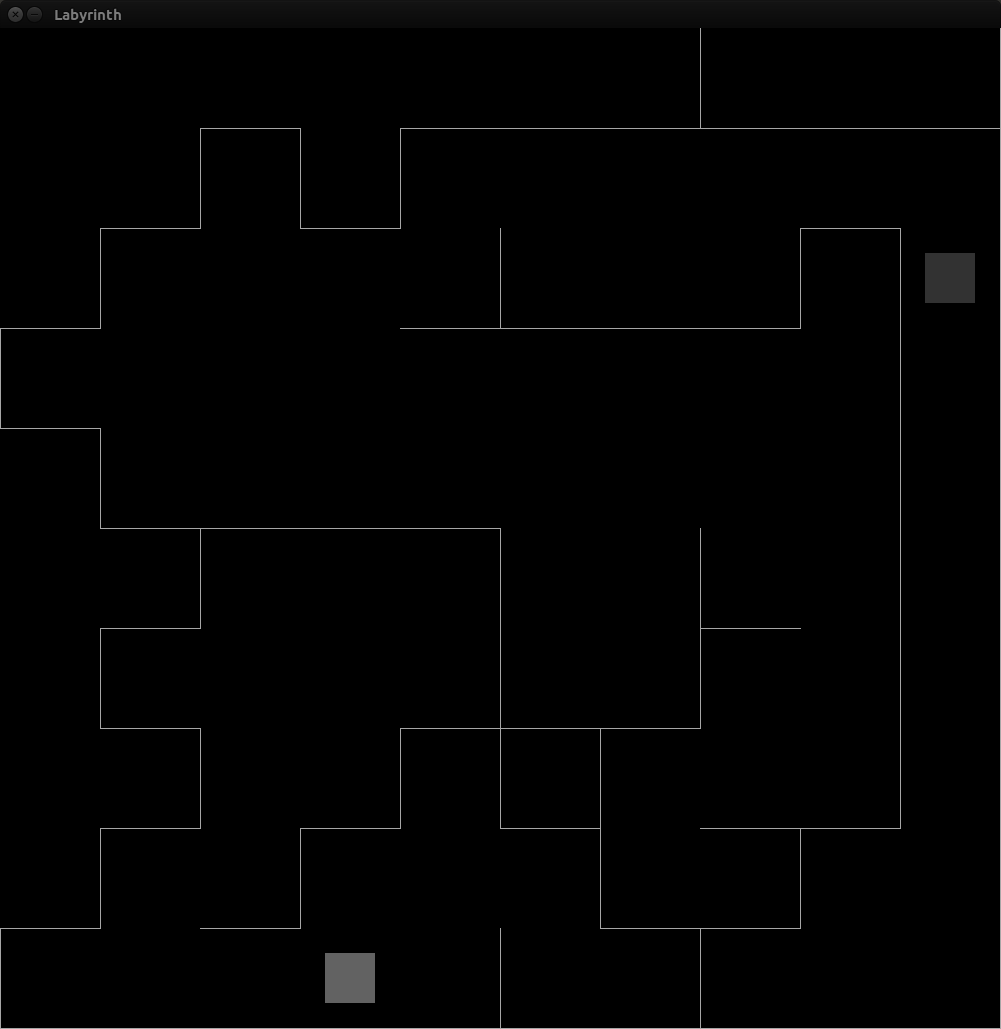
\includegraphics[width=1\linewidth]{2-4}}\\
	\end{minipage}
	\hfill
	\begin{minipage}[h]{0.3\linewidth}
		\center{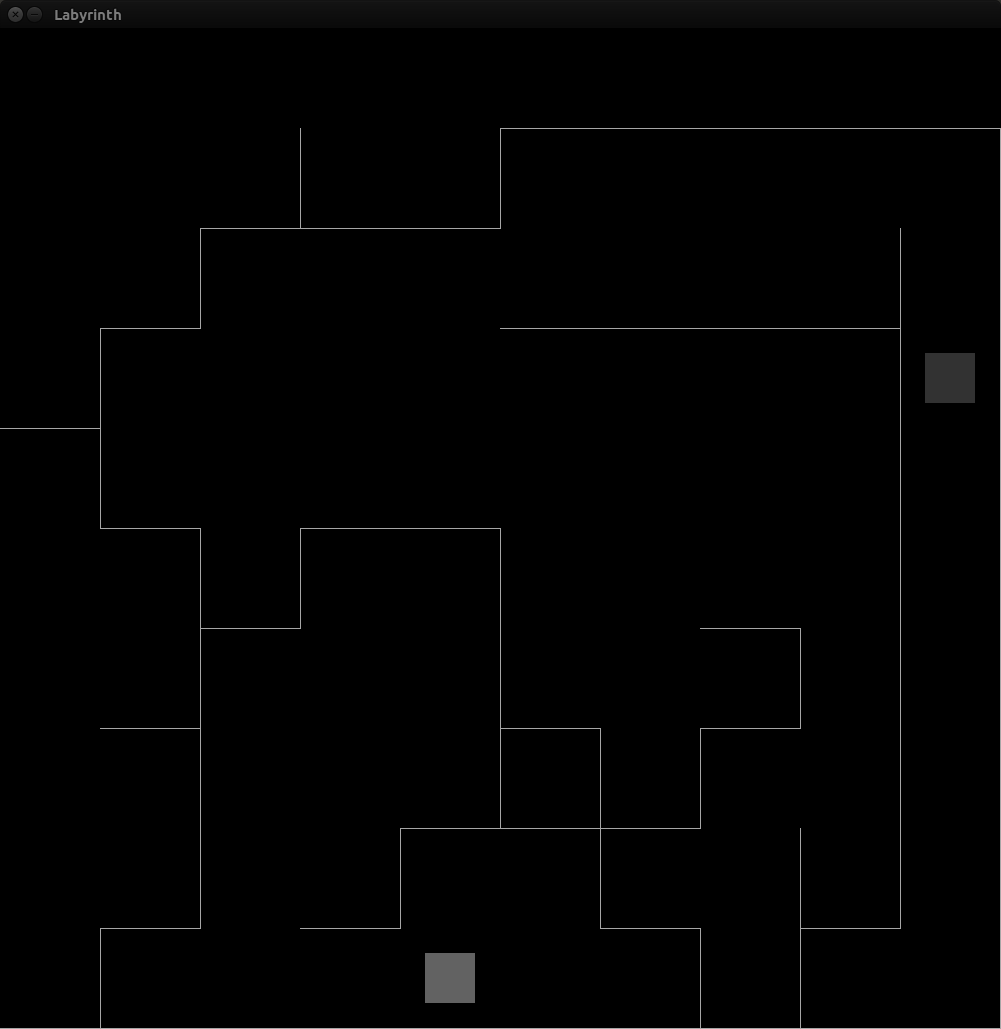
\includegraphics[width=1\linewidth]{2-5}}\\
	\end{minipage}
	\hfill
	\begin{minipage}[h]{0.3\linewidth}
		\center{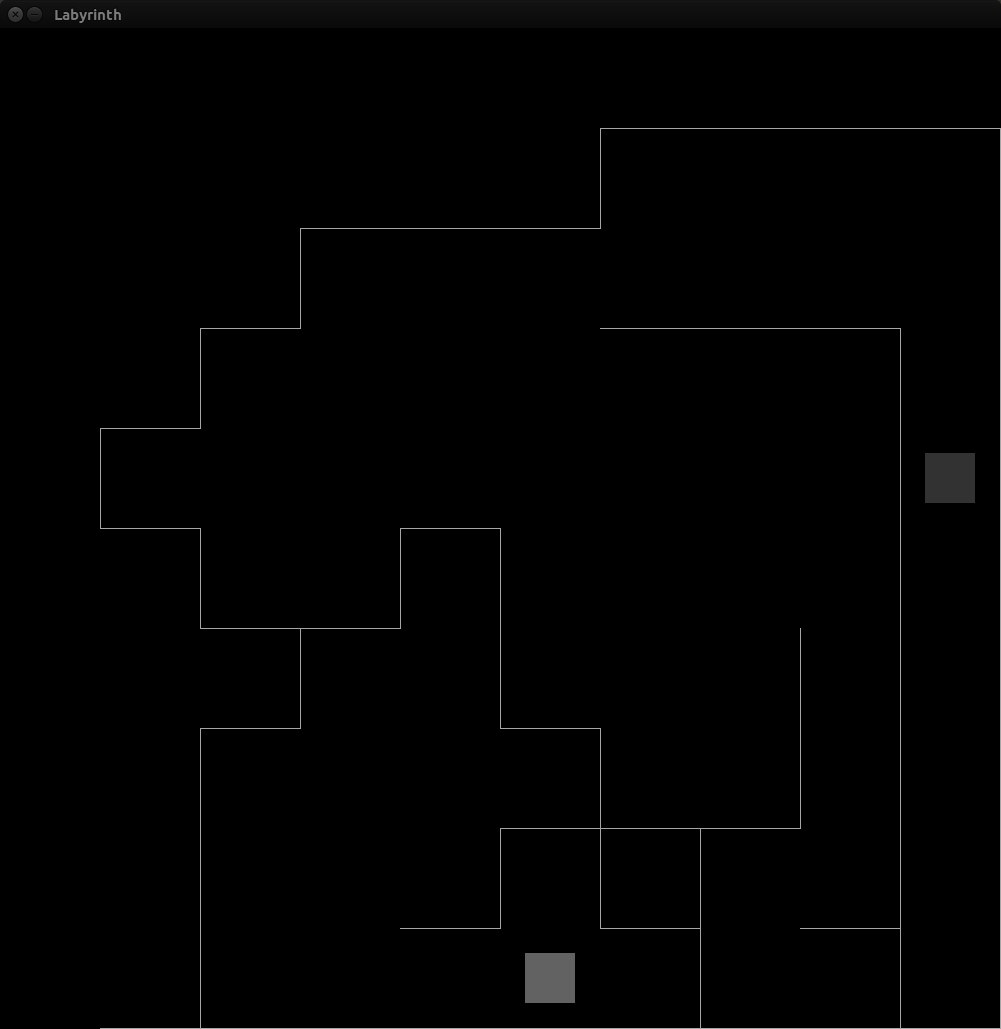
\includegraphics[width=1\linewidth]{2-6}}\\
	\end{minipage}
	\hfill
	\begin{minipage}[h]{0.3\linewidth}
		\center{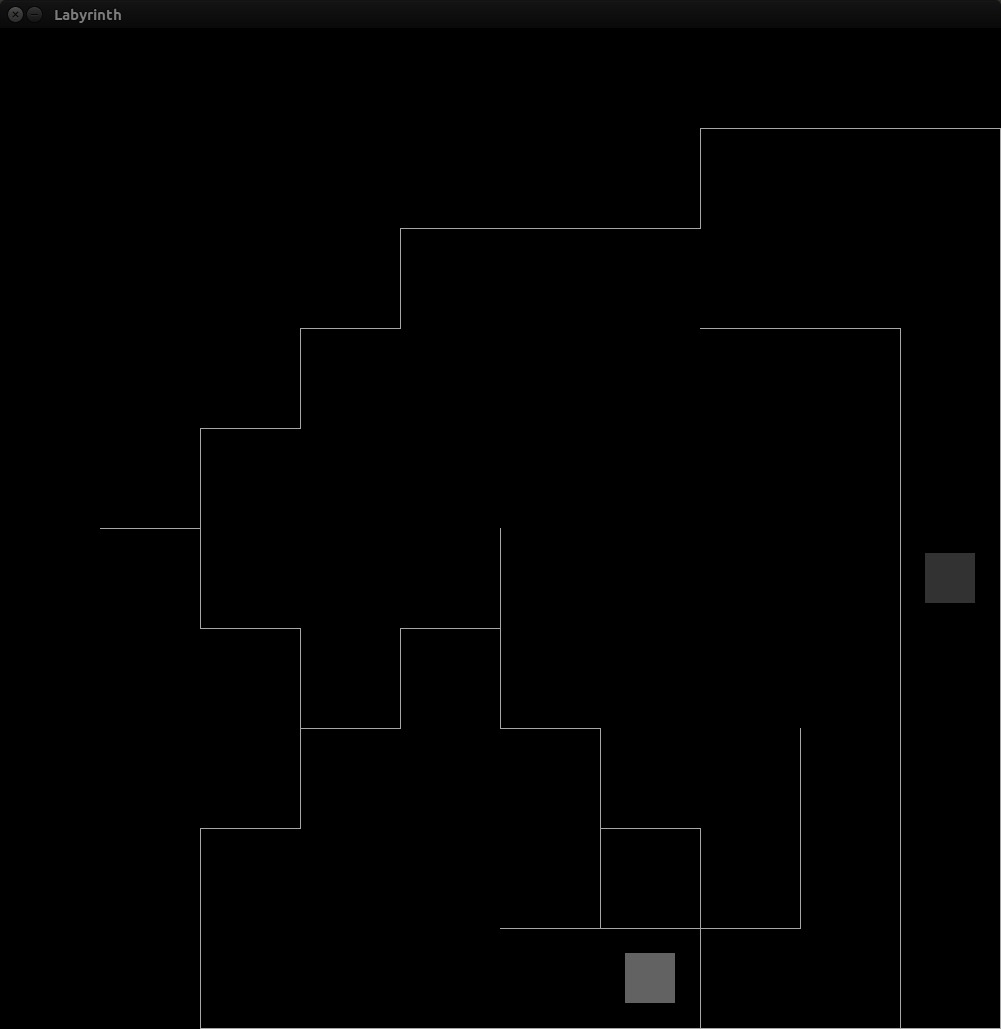
\includegraphics[width=1\linewidth]{2-7}}\\
	\end{minipage}
	\hfill
	\begin{minipage}[h]{0.3\linewidth}
		\center{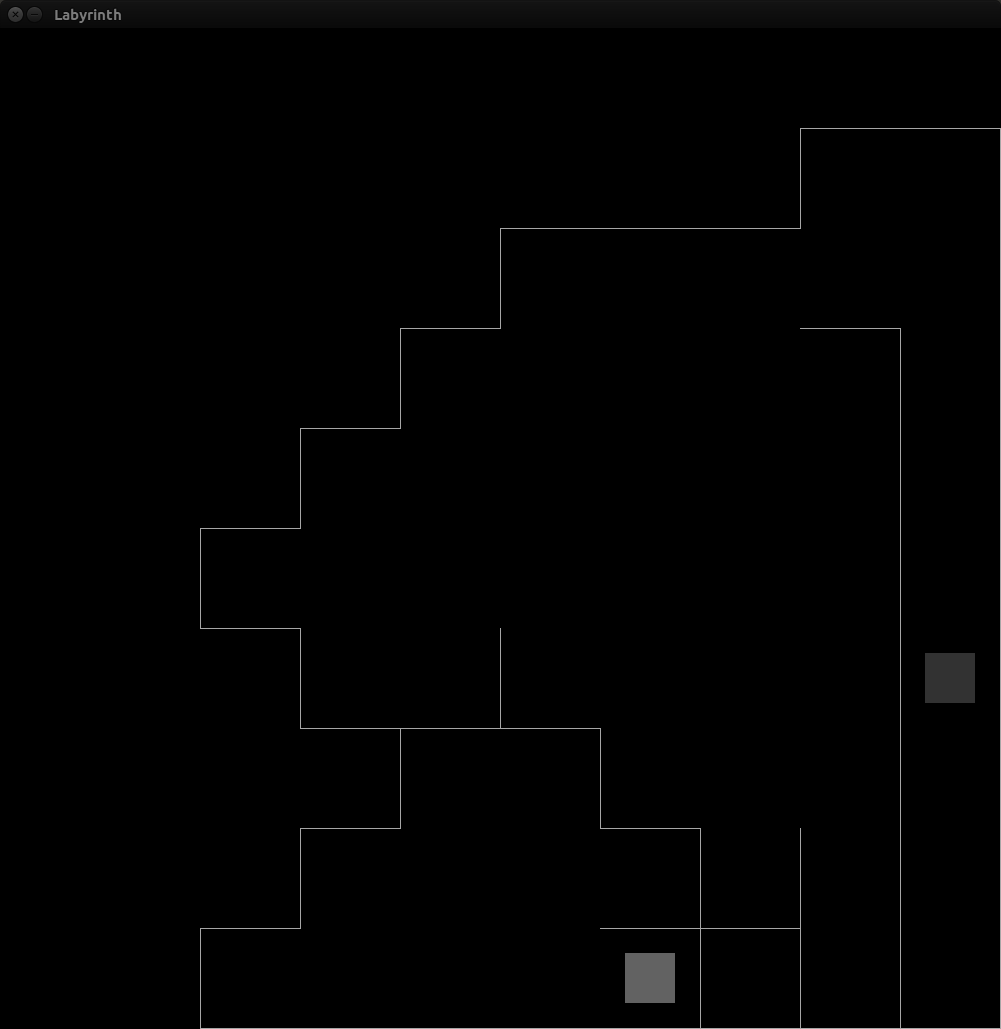
\includegraphics[width=1\linewidth]{2-9}}\\
	\end{minipage}
	\hfill
	\begin{minipage}[h]{0.3\linewidth}
		\center{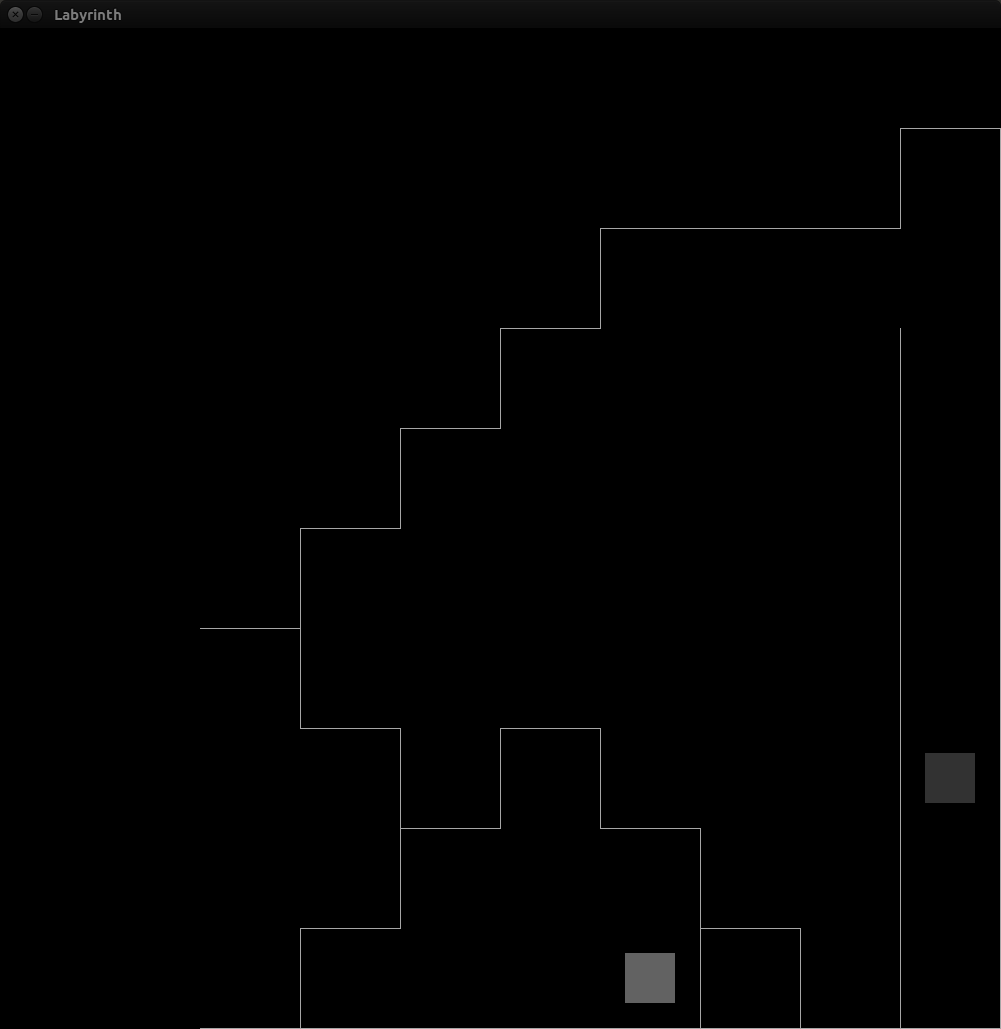
\includegraphics[width=1\linewidth]{2-10}}\\
	\end{minipage}
	\hfill
	\begin{minipage}[h]{0.3\linewidth}
		\center{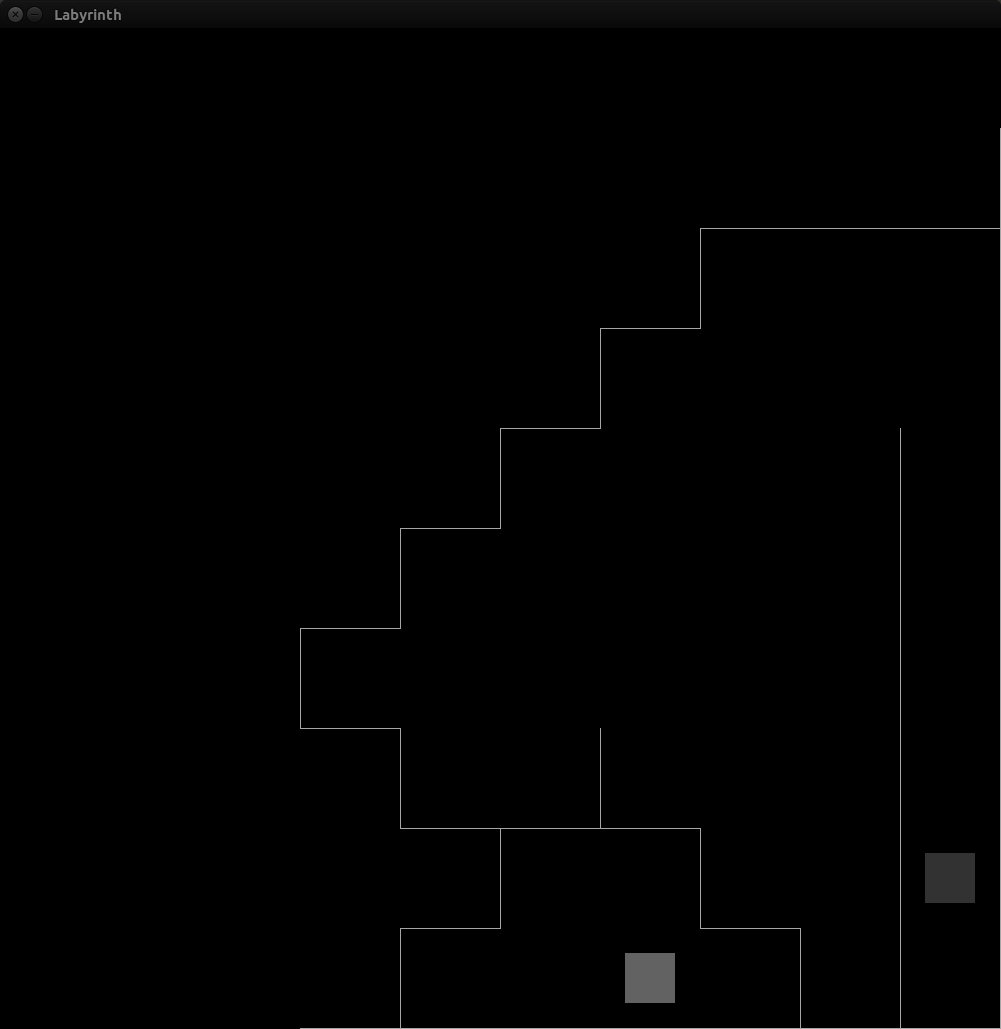
\includegraphics[width=1\linewidth]{2-11}}\\
	\end{minipage}
	\hfill
	\begin{minipage}[h]{0.3\linewidth}
		\center{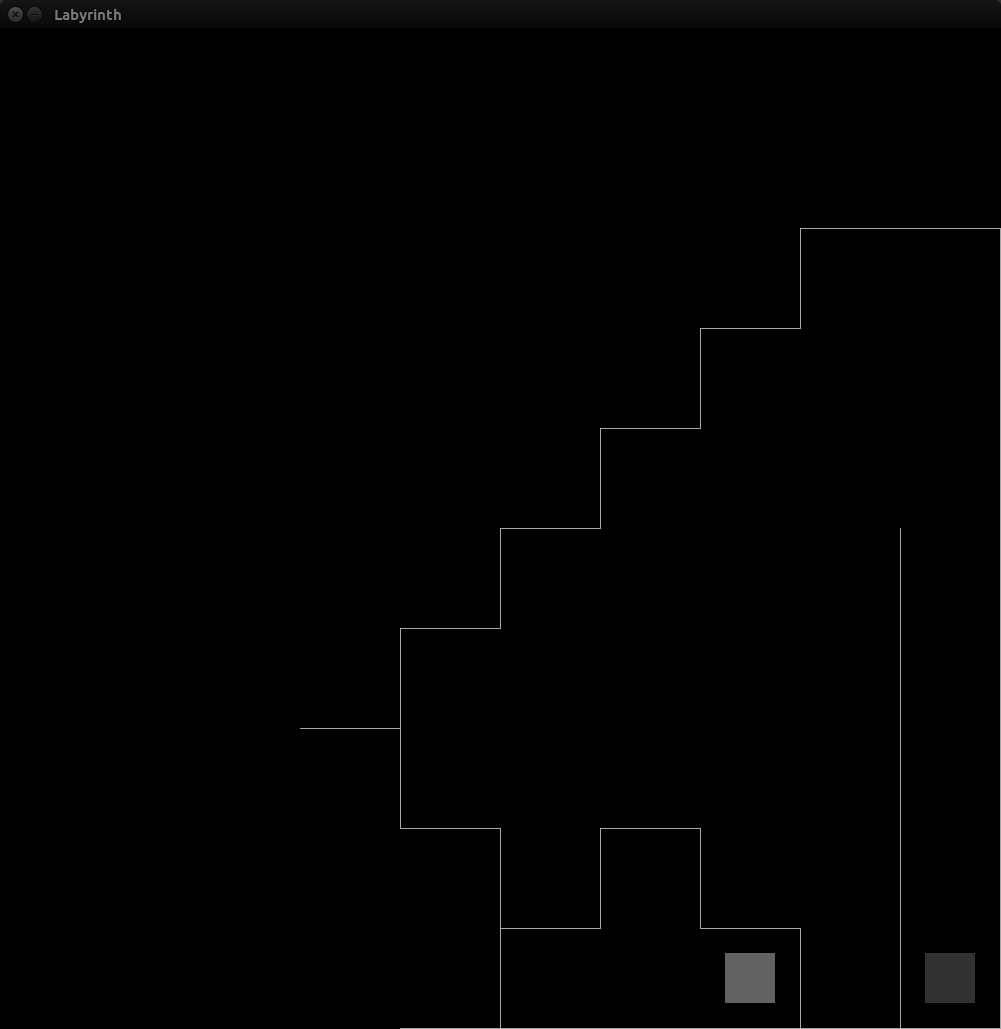
\includegraphics[width=1\linewidth]{2-12}}\\
	\end{minipage}
	\hfill
	\begin{minipage}[h]{0.3\linewidth}
		\center{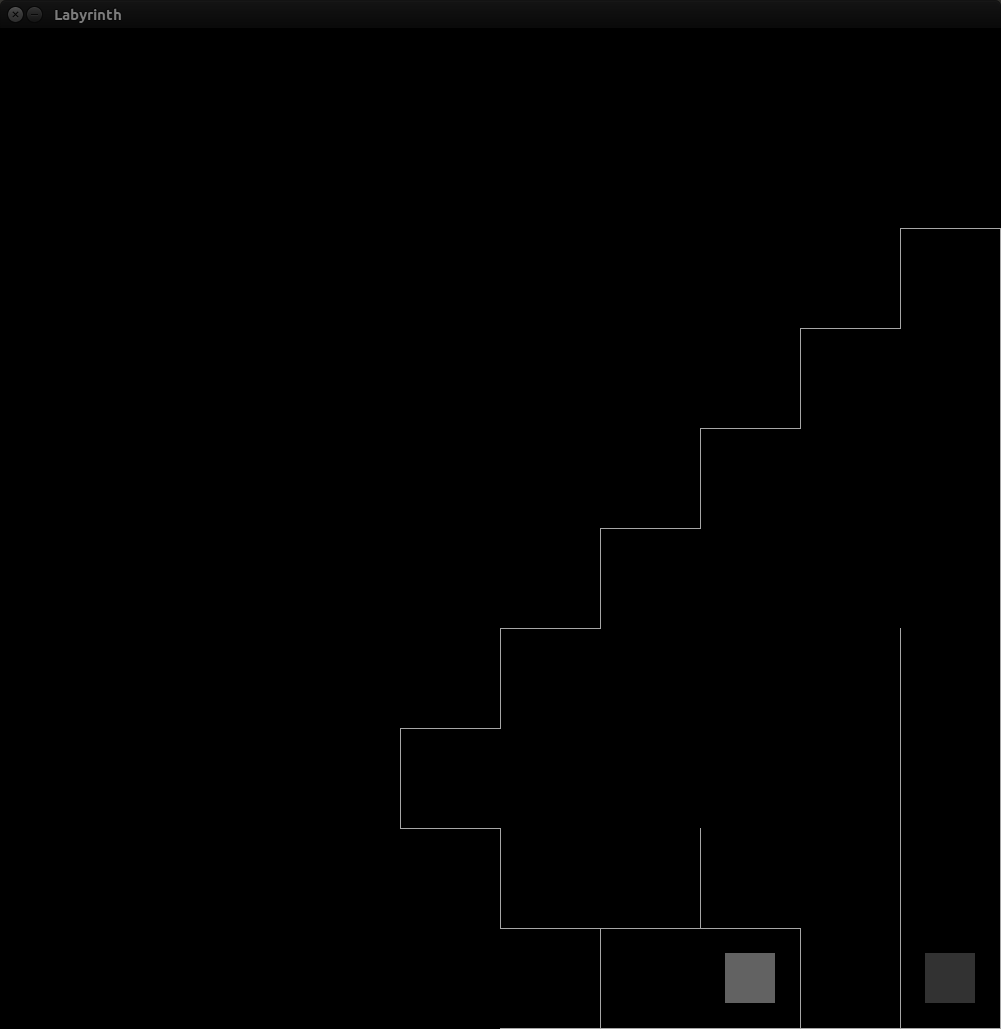
\includegraphics[width=1\linewidth]{2-13}}\\
	\end{minipage}
	\hfill
	\begin{minipage}[h]{0.3\linewidth}
		\center{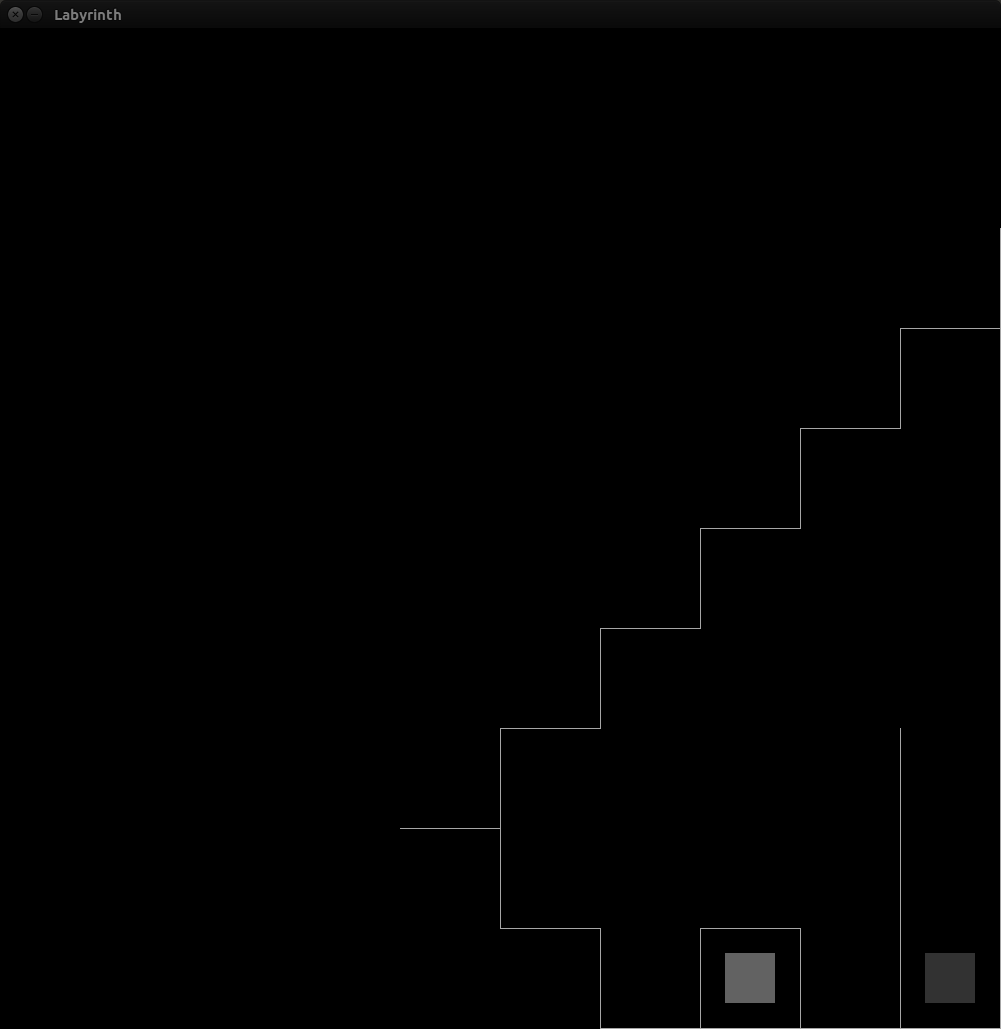
\includegraphics[width=1\linewidth]{2-14}}\\
	\end{minipage}
	\hfill
	\caption{Пример работы алгоритма(Пути нет)}
	\label{fig:ex_2}
\end{figure}

\section*{Корректность алгоритма}
Покажем, что если существует путь из $A$ в $B$, то он не исчезает при работе алгоритма.

\begin{claim*}
	Если клетки $A$ и $B$ принадлежат одной компоненте связности, то после каждого шага алгоритма, они будут оставаться связными.
\end{claim*}
\begin{proof}[Доказательство]
	Воспользуемся доказательством от противного. Пусть на некотором шаге алгоритма, старт и финиш располагались в одной компоненте связности, а на следующем шаге, путь из $A$ в $B$ перестал существовать. Заметим, что путь может исчезнуть только при добавлении стенок. Из указанных нами правил добавление стенок происходит только по правилу $2$, которое изменяет клетки с левым верхним уголком. Таким образом, если между $A$ и $B$ существовал путь, не проходящий через такие клетки, то путь сохранится и в лабиринте на следующем шаге. Значит, из нашего предположения следует, что исходные пути из $A$ в $B$ содержат левый верхний уголок. Докажем, что правила преобразования изменяют лабиринт, таким образом, что появляется обходной путь из $A$ в $B$.
	
	\bigskip
	
	Вначале рассмотрим случай, когда уголок не явлется стартом/ финишем. Поскольку, предполагается, что клетка с уголком является частью пути, делаем вывод, что правая и нижняя стенки открыты. На рис. \ref{fig:alt_way} показаны все возможные, ситуации в окрестности и уголка и конфигурации этой окрестности после применения правил. Легко видеть, что хоть мы и исключили уголок из пути, но при этом появился "обход" через клетку справа-снизу относительно уголка. Таким образом, добавление новых стенок не нарушила связности старта и финиша.
	
	\begin{figure}[H]
	 	  \centering
          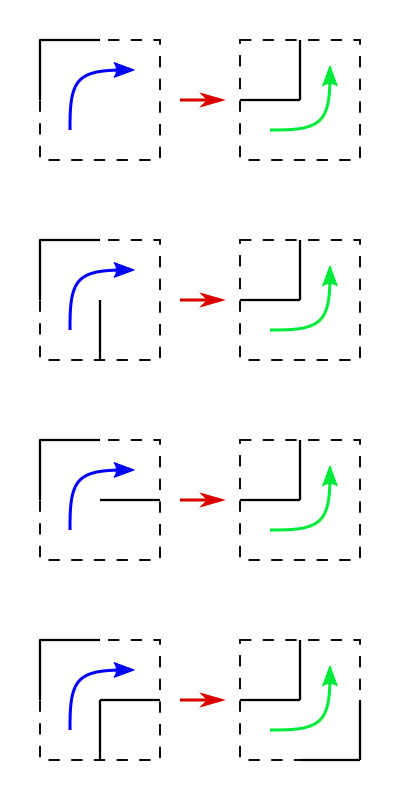
\includegraphics[width=0.25\linewidth]{another_way}
          \caption{Изменение схемы лабиринта, с возникающим обходом(штрихом указаны отрезки состояния, которых неизвестны)}
         \label{fig:alt_way}
     \end{figure}
	
	Рассмотрим теперь случай, когда уголок является стартом или финишем. Поскольку существует некоторый путь, то либо правая, либо нижняя стенка открыты. По 3-му правилу старт/финиш переместится по возможности вниз, а если это невозможно -- вправо. Если при этом старт/финиш окажется в следующей/предыдущей клетке "старого" пути, то в силу доказанного ранее, путь из $A$ в $B$ по-прежнему будет существовать. Если же, старт/финиш переместились в клетку, которая не была частью пути(то есть сместились вниз, когда старый путь шёл вправо/справа, заметим, что при этом и правая и нижняя стенка должны быть открыты, как и в первой части доказательства), то по \ref{fig:alt_way}  видно, что существует возможность добраться в клетку "старого" пути.
	
	\bigskip
	
	Таким образом, мы показали, что правила лабиринта изменяют его так, что расположние клеток $A$, $B$ относительно компонент связности не изменяется.
\end{proof}

Далее покажем, что если пути между $A$ и $B$ не существовало, то изменения лабиринта не приведут к его появлению.
\begin{claim*}
	Если клетки $A$ и $B$ принадлежат разным компонентам связности, то на каждом шаге алгоритма, эти клетки будут принадлежать разным компонентам.
\end{claim*} 
\begin{proof}[Доказательство.]
	Появление пути означает, что две клетки лабиринта ранее принадлежащие разным компонентам свяязности теперь принадлежат одной. Мы покажем, что наши правила исключают возможность присоединения клетки с сохранением связности со своей предыдущей компонентой.

	Заметим, что первое правило удаляет стенку между клетками одной компоненты(так как одиночную стенку, очевидно, можно обойти). То есть как и в предыдущем доказательстве, мы рассматриваем клетки, к которым применяется второе правило. Будем вначале предполагать, что старт/ финиш не меняют своих клеток. На рис. \ref{fig:split} показаны, все возможные конфигурации отщепляемой клетки от компоненты связности и их состояния при преобразовании. Как видно из рисунка, клетка присоединяясь к одной компоненте связности отгараживается от ранее смежных с ней клеток. Таким образом, через эту клетку не может проходить путь из компоненты финиша в компоненту старта. Поэтому единственный вариант, появления пути, что сама клетка финиша или старта была перемещена в другую компоненту связности. Покажем, что и этого не могло произойти.
	
	\begin{figure}[H]
	 	  \centering
          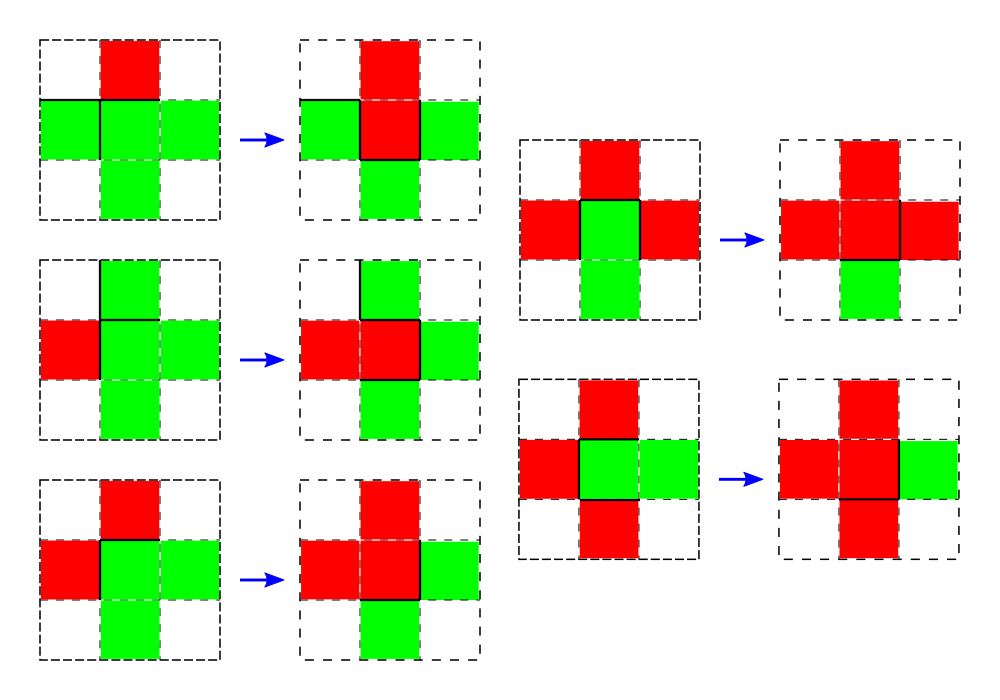
\includegraphics[width=0.8\linewidth]{split}
          \caption{Клетка, меняющая компоненту связности. Одинаковым цветом выделены клетки которые могут лежать в одной компоненте свзяности, разными -- точно разные компоненты связности}
         \label{fig:split}
     \end{figure}
     
$1$-й случай: старт/финиш лежит в клетке с правым нижним уголком. В этом случае старт/финиш не смещается. Такая клетка не содержит  левый верхний уголок(так как иначе это было бы состояние принятия решения) и, следовательно, не открывает стенки(кроме одиночных, но как уже упоминалось их удаление не меняет компоненты связности). 

$2$ - случай -- клетка не содержит правый нижний. В этом случае, старт/финиш смещается в клетку(заметим, не содержащую левый верхний уголок). Поэтому компонента связности сохраняет старые клетки, за исключением, возможно, некоторых клеток, содержащих левый верхний уголок. Последние же как было показано раннее, при смене компоненты изолируются от бывших соседей, поэтому слияния компонент не происходит.
\end{proof}

Итак, мы доказали, что если между $A$ и $B$ существовал путь, то в преобразованном лабиринте путь тоже будет существовать. Если же пути не было, то он не появится. Следовательно, в силу уменьшения объёма лабиринта(данный факт, будет доказан в следующем пункте) одно из состояний принятия решения будет достигнуто, а доказанные утверждения означают, что полученный результат -- корректен.

В следующем пункте, мы покажем, что алгоритм работает за $O(n)$ тактов.

\section*{Время работы алгоритма}

Напомним, что в конце первого пункта мы условились "вкладывать" данный нам лабиринт в "кожух" из слоя пустых клеток.

\begin{claim*}
	На каждом шаге алгоритма количество клеток, принадлежащих лабиринту уменьшается, остальные присоединяются к "кожуху. Алгоритм завершится не более чем за $2n$ итераций клеточного автомата.
\end{claim*}
\begin{proof}
	Рассмотрим левую верхнюю клетку лабиринта. Она содержит левый верхний уголок. После применения $2$-го правила эта клетка становится частью кожуха(появляются правая и нижняя стенки, старые -- удаляются). При этом появляются два левых верхних уголка. На следующем шаге эти два уголка добавятся к кожуху, появтся новые три. Продолжая эти действия (см.\ref{fig:steps}) видим, что за $n$ шагов, лбиринт будет заключён в правом нижнем треугольнике исходного лабиринта(с каждым шагом из верхнего ряда исключается одна клетка лабиринта). Ещё через $n$ шагов, лабиринт свернётся в клетку (если до этого не произошло событие принятия решения). Так как все правила сохраняют старт и финиш внутри лабиринта, в этот момент они окажутся в одной клетке, что является событием принятия решения. 
	
	\begin{figure}[H]
	 	  \centering
          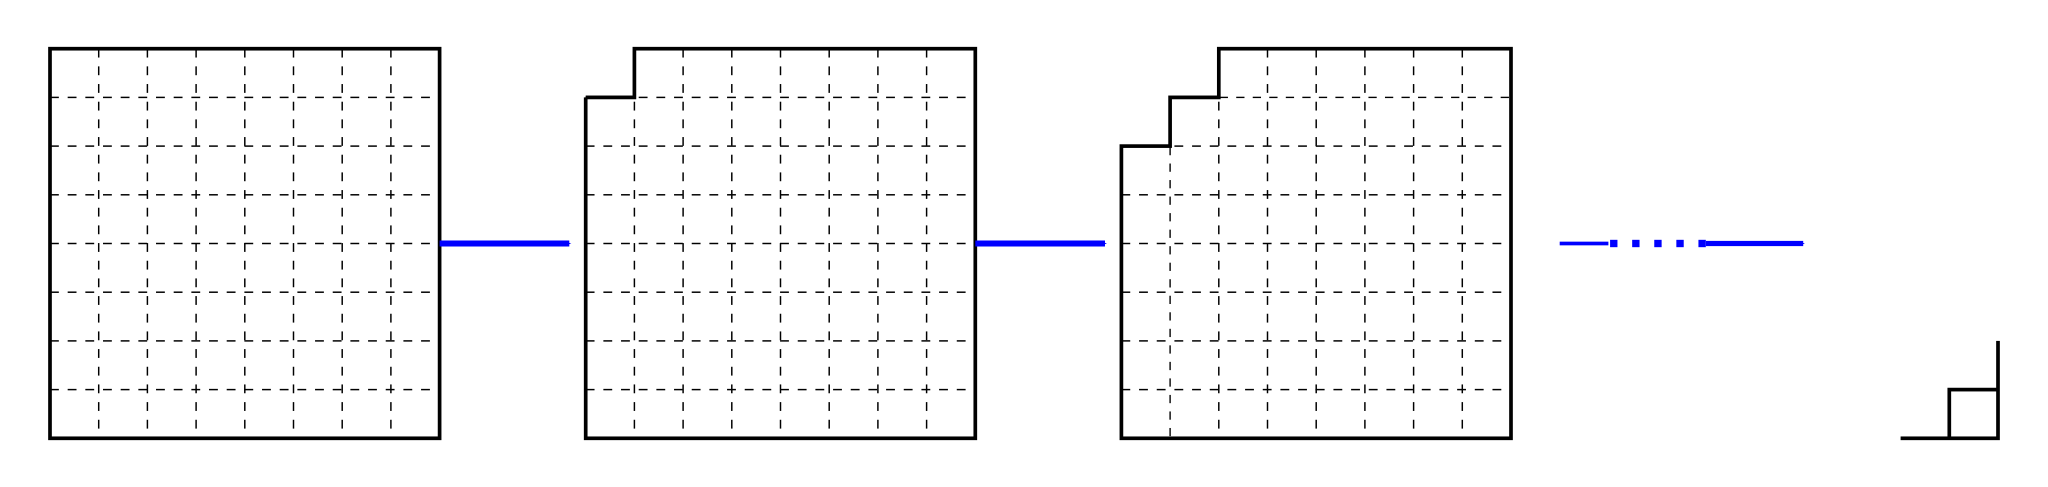
\includegraphics[width=0.8\linewidth]{steps}
          \caption{"Сворачивание" лабиринта}
         \label{fig:steps}
     \end{figure}
     
Отметим, что сворачивание лабиринта  происходит назависимо от его содержимого, то есть конфигурация лабиринта не может задерживать свёртку и не более чем через $2n$ операций  перейдёт в состояние принятия решения. 
\end{proof}

Итак, мы доказали корректность алгоритма и сложность его работы. Тем самым мы подтвердили, что алгоритм удовлетворяет условию задачи.

Наконец, покажем принципиальную невозможность существования алгоритма, решающий поставленную задачу за $o(n)$ тактов.

\section*{Несуществование корректного алгоритма o(n)}

\begin{claim*}
	Не существует корректного алгоритма, решающего поставленную задачу, сложности $o(n)$
\end{claim*}
\begin{proof}
	Рассмотрим произвольный корректный алгоритм, решающий задачу. Запустим его на трёх схожих лабиринтах, отличающихся наличием отсутствием двух стенок(см. рис \ref{fig:unsolved})
	
	Как видно из рисунка в случаях $a)$ и $b)$ путь из  $A$ в $B$ существует. Клетками $1,2$ помеченны клетки состояние которых может отличаться от состояний тех же клеток в других лабиринтах (если клетка в разных лабиринтах обозначена одной цифрой -- их состояния совпадают). Так как пути существуют, ни одна из клеток, помеченных цифрами не может быть состоянием принятия отрицательного решения(то есть состояние которое означает, что в лабиринте нет пути).
	
	Обратимся теперь к лабиринту $c)$. Очевидно, в нём пути не существует. При этом клетки инициализированы так же как и в лабиринтах, где пути нет. Это означает, что пока "возмущение" от клеток расположенных у т-образных соединений не наложатся(при этом состояние клетки, в которой произошло наложение неопределенно и может быть состоянием, соответствующим отсутствию пути в лабиринте), алгоритм не завершит работу. Но наложение произойдёт через $n/2$ тактов. То есть количество тактов алгоритма ограниченно снизу $n/2$, откуда следует $T(n) \neq o(n)$
	
	\begin{figure}[H]
	 	  \centering
          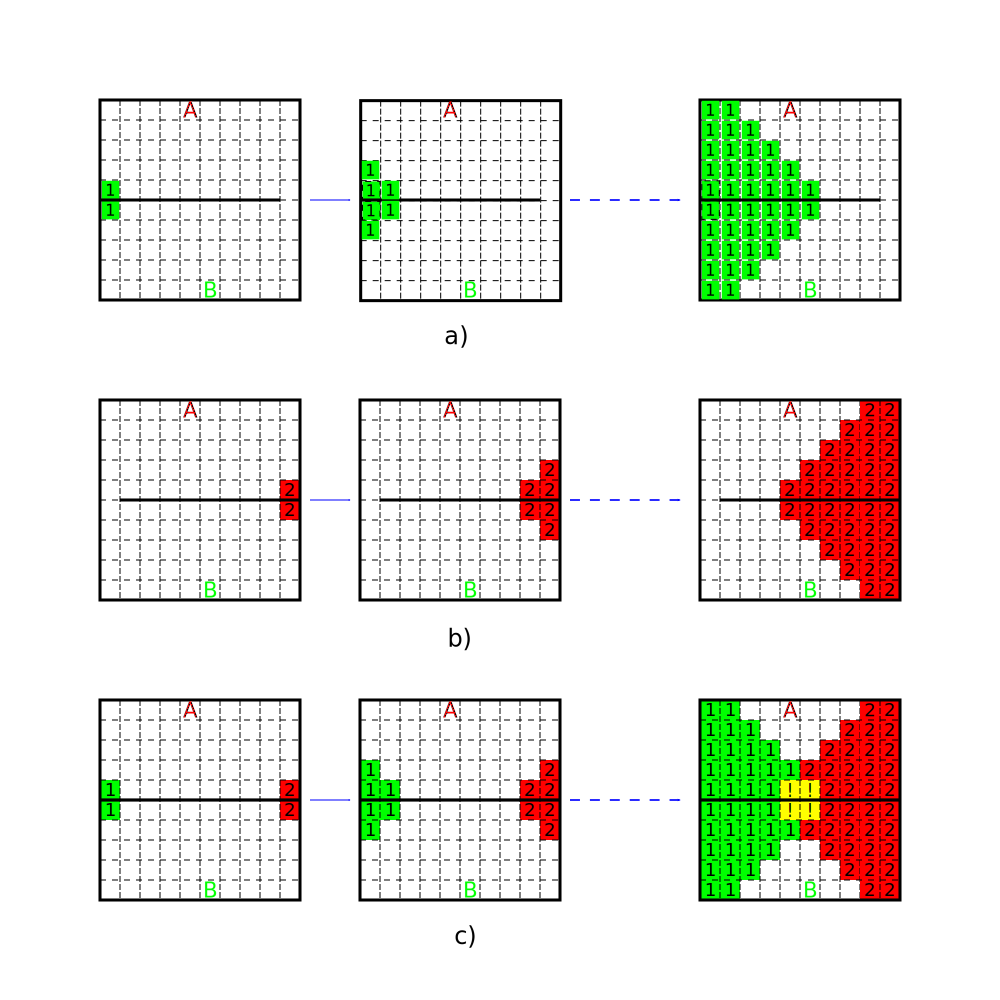
\includegraphics[width=0.8\linewidth]{unsolved}
          \caption{Изменение состояний клеток в процессе выполнения алгоритма. Цифрами и пустыми клетками отмечены клетки, состояние которых не означают отсутствие пути в лабиринте, состояние жёлтых клеток неопределенно и может приводить к завершению алгоритма}
         \label{fig:unsolved}
     \end{figure}
\end{proof}
\end{document}